%using document class from KOMA-Script
\documentclass{scrartcl}
\title{M1J1 Summary Notes}
\subtitle{JMC Year 1, 2017/2018 syllabus}
\date{}
\author{Fawaz Shah (original notes by Dr Berkshire and Dr Lawn)}

% Packages for adding hyperlinks to table of contents
\usepackage{color}   %May be necessary if you want to color links
\usepackage{hyperref}
\hypersetup{
    colorlinks=true, %set true if you want colored links
    linktoc=all,     %set to all if you want both sections and subsections linked
    linkcolor=black,  %choose some color if you want links to stand out
}

%package that allows aligned equations
\usepackage{amsmath}

%package that allows notation for extra mathematical symbols
\usepackage{amssymb}

%new commands for popular sets for ease of use
\newcommand{\R}{\mathbb{R}}
\newcommand{\N}{\mathbb{N}}
\newcommand{\Z}{\mathbb{Z}}
\newcommand{\Q}{\mathbb{Q}}
\newcommand{\C}{\mathbb{C}}

% renaming command to writing vectors in bold notation
\renewcommand{\vec}[1]{\mathbf{#1}}

%package for managing images
\usepackage{graphicx}
\graphicspath{ {../img/} }

%package for managing hyperlinks
\usepackage{hyperref}

%package for added blue colored boxes
\usepackage[most]{tcolorbox}

%package that allowed removing indent from enumerate environment
\usepackage{enumitem}

%package that allows for negating nearly any symbol
\usepackage{centernot}

\usepackage{relsize}

\begin{document}
\large
\maketitle
\begin{center}
UNDER CONSTRUCTION
\end{center}
\noindent The structure of this document is split since the two parts were taught by different lecturers.
\\\\
Note that the exam will probably require you to PROVE some of these theorems, so you should refer back to the original notes for the proofs.
\\\\
Boxes cover content in more detail. Titles of some theorems are given in italics.
\tableofcontents
\newpage
\part{Applied Methods}

\section{Definitions}

\paragraph{Order (of derivative)}
An $ n^{th} $ derivative has order $ n $.

\paragraph{Order (of ODE)}
The order of the highest derivative present in an ODE.

\paragraph{Degree (of ODE)}
The highest power to which a term is raised in an ODE (excluding fractional powers).

\paragraph*{Linear (ODE)}
An ODE which has no terms raised to more than the $ 1^{st} $ power, and with no $ y, x $ or other derivative terms multiplied by each other.

\paragraph{System of diff. equations}
A set of simultaneous equations of derivatives, where derivatives of $ y, x $ etc. are given w.r.t. a parameter $ t $

\paragraph{Order (of system)}
The order of the highest derivative present in the system.

\paragraph{Degree (of system)}
The highest power to which a term is raised in an ODE (excluding fractional powers).

\paragraph{Linear (system)}
A system which has no terms raised to more than the $ 1^{st} $ power, and with no $ y $ or other derivative terms multiplied by each other.

\paragraph{Homogeneous (system)}
A system with no explicit functions of $ t $ present.

\paragraph{Order (difference equation)}
The order of a recurrence relation for $ u_{n} $ is the number of previous $ u_{n} $ terms it relates to.

\paragraph{Linear (difference equation)}
A recurrence relation for $ u_{n} $ is linear if it only contains $ u_{n} $ terms to the $ 1^{st} $ power, and has no $ u_{n} $ terms multiplied by each other.

\paragraph{Homogenous (difference equation)}
A recurrence relation for $ u_{n} $ is homogenous if there are no explicit functions of $ n $ present.

\paragraph{Forward difference operator $ \Delta $}
The forward difference operator is defined as:
\begin{equation}
\Delta U(n) = U(n+1) - U(n)
\end{equation}

\paragraph{Newton-Raphson method}
The Newton-Raphson iterative formula to find $ x $ such that $ f(x) = 0 $ is:
\begin{equation}
x_{n+1} = x_{n} - \frac{f(x_{n})}{f'(x_{n})}
\end{equation}
Note that this only works in specific cases.

\paragraph{Taylor series (multivariable)}
The Taylor series centered around $ (a, b) $ for a multivariable function $ f(x, y) $ can be written as:
\begin{align}
f(x, y) & = \color{cyan}{f(a, b)} + \color{blue}{f'_{x}(a, b)(x-a) + f'_{y}(a, b)(y-b)} \\
& + \color{magenta}{\frac{1}{2!}(f''_{xx}(a, b)(x-a)^{2} + 2f''_{xy}(a, b)(x-a)(y-b)} \\
& \ \ \ \color{magenta}{ + f''_{yy}(a, b)(y-b)^{2})} \color{black}{\textrm{ + ...}}
\end{align}
where:
\begin{equation}
f'_{x} = \frac{\partial f}{\partial x}, \quad f''_{xx} = \frac{\partial^{2} f}{\partial x^{2}}, \quad f''_{xy} = \frac{\partial^{2} f}{\partial x \partial y} = \frac{\partial^{2} f}{\partial y \partial x}\textrm{ ... etc.}
\end{equation}
If we let $ h = x - a $ and $ k = y - b $ then we can also write the Taylor series as:
\begin{align}
f(a+h, b+k) & = \color{cyan}{f(a, b)} + \color{blue}{hf'_{x}(a, b) + kf'_{y}(a, b)} \\
& + \color{magenta}{\frac{1}{2!}(h^{2}f''_{xx}(a, b) + 2hkf''_{xy}(a, b) + k^{2}f''_{yy}(a, b))} \color{black}{\textrm{ + ...}}
\end{align}

\paragraph{Exact (total) differential}
The exact differential of a multivariable function $ f(x, y) $ is the equation:
\begin{equation}
df = dx \frac{\partial f}{\partial  x} + dy \frac{\partial f}{\partial  y}
\end{equation}

\paragraph{Exact equation}
A differential equation of the form:
\begin{equation} \label{exacteq}
P(x, y) + Q(x, y) \frac{dy}{dx} = 0
\end{equation}
is called an exact equation iff:
\begin{equation}
\frac{\partial P}{\partial y} \equiv \frac{\partial Q}{\partial x}
\end{equation}
Note that in this case the LHS of equation \ref{exacteq} forms an exact differential, which can be used to to find the general solution (explained later on).

\paragraph{Scalar field}
A function that associates a scalar value to every point in (3D) space.

\paragraph{Vector field}
A function that associates a vector to every point in (3D) space.

\paragraph{Partial differential operator $ \nabla $}
Imagine we have a 3D vector field with standard basis vectors $ \vec{i}, \vec{j} $ and $ \vec{k}  $. We define the operator $ \nabla $ to be:
\begin{equation}
\nabla = \vec{i} \frac{\partial}{\partial x} + \vec{j} \frac{\partial}{\partial y} + \vec{k} \frac{\partial}{\partial z}
\end{equation}

\paragraph{grad}
The gradient (grad) of a scalar field produces a vector field. For a scalar field $ \phi(x, y, z) $ we denote the grad as $ \nabla \phi $. At any point in space, grad is defined as:
\begin{equation}
\nabla \phi = \frac{\partial \phi}{\partial x} \vec{i} + \frac{\partial \phi}{\partial y} \vec{j} + \frac{\partial \phi}{\partial z} \vec{k}
\end{equation}

\paragraph{div}
The divergence (div) of a vector field produces a scalar field. For a vector field $ \vec{u}(x, y, z) $ we denote the div as $ \nabla \cdot \vec{u} $. At any point in space, div is defined as:
\begin{equation}
\nabla \cdot \vec{u} = \frac{\partial u_{1}}{\partial x} + \frac{\partial u_{2}}{\partial y} + \frac{\partial u_{3}}{\partial z}
\end{equation}
where $ \begin{pmatrix}
u_{1} \\ u_{2} \\ u_{3}
\end{pmatrix} $ is the value of $ \vec{u} $ at that point.

\paragraph{curl}
The curl of a vector field produces a vector field. For a vector field $ \vec{u}(x, y, z) $ we denote the curl as $ \nabla \times \vec{u} $. At any point in space, curl is defined as:
\begin{align}
\nabla \times \vec{u} & = \det \begin{pmatrix}
\vec{i} & \vec{j} & \vec{k} \\
\frac{\partial}{\partial x} & \frac{\partial}{\partial y} & \frac{\partial}{\partial z} \\
u_{1} & u_{2} & u_{3}
\end{pmatrix} \\\\
& = (\frac{\partial u_{3}}{\partial y} - \frac{\partial u_{2}}{\partial z})\vec{i} + (\frac{\partial u_{3}}{\partial x} - \frac{\partial u_{1}}{\partial z})\vec{j} + (\frac{\partial u_{2}}{\partial x} - \frac{\partial u_{1}}{\partial y})\vec{k}
\end{align}
where $ \begin{pmatrix}
u_{1} \\ u_{2} \\ u_{3}
\end{pmatrix} $ is the value of $ \vec{u} $ at that point.

\section{2nd order ODEs}

\subsection{Special case - y missing}
If we can write the $ 2^{nd} $ derivative in the form:
\begin{equation}
\frac{d^{2}y}{dx^{2}} = f(x, \frac{dy}{dx})
\end{equation}
(i.e. no $ y $ terms present), then we can make a substitution. Let $ P = \frac{dy}{dx} $. This means $ \frac{d^{2}y}{dx^{2}} = \frac{dP}{dx} $, the
refore we have:
\begin{equation}
\frac{dP}{dx} = f(x, P)
\end{equation}
This is 1st order w.r.t P and can be solved by appropriate 1st order methods.

\subsection{Special case - x missing}
If we can write the $ 2^{nd} $ derivative as:
\begin{equation}
\frac{d^{2}y}{dx^{2}} = f(y, \frac{dy}{dx})
\end{equation}
(i.e. no x terms present), then we can make the same substitution. Let $ P = \frac{dy}{dx} $. This means $ \frac{d^{2}y}{dx^{2}} = \frac{dP}{dx} $, therefore we have:
\begin{equation}
\frac{dP}{dx} = f(y, P)
\end{equation}
However, this is not yet a 1st order equation since the derivative is w.r.t. x, but we only have y terms on the RHS.
\\\\
DIFFERENT TO LAST TIME: we must rewrite $ \frac{dP}{dx} $ as a derivative with respect to y. Luckily, we can see that:
\begin{equation}
\frac{dP}{dx} = \frac{dP}{dy}\frac{dy}{dx} = P\frac{dP}{dy}
\end{equation}
Therefore:
\begin{equation}
P\frac{dP}{dy} = f(y, P)
\end{equation}
This is 1st order w.r.t P and can be solved by appropriate 1st order methods.

\subsection{Finding the CF}
The general solution (GS) of a 2nd order ODE can be expressed as the sum of two other functions, called the \textbf{complementary function} (CF) and the \textbf{particular integral} (PI).
\begin{equation}
y_{GS} = y_{CF} + y_{PI}
\end{equation} 
A 2nd order ODE will usually be presented to us in the form:
\begin{equation} \label{generalformdifferential}
a\frac{d^{2}y}{dx^{2}} + b\frac{dy}{dx} + c = f(x)
\end{equation}
It can be shown that the CF can be calculated from the LHS of the above equation. We write down the \textbf{auxiliary equation}, which is simply the equation:
\begin{equation}
a\lambda^{2} + b\lambda + c = 0
\end{equation}
using a, b, c from above. Solving this gives us two values, $ \lambda_{1} $ and $ \lambda_{2} $.

\subsubsection*{Case 1: $ \lambda_{1} \neq \lambda_{2} $, both real}
We can express the CF as:
\begin{equation}
y_{CF} = A_{1}e^{\lambda_{1}x} + A_{2}e^{\lambda_{2}x}
\end{equation}
where $ A_{1} $ and $ A_{2} $ are arbitrary constants.

\subsubsection*{Case 2: $ \lambda_{1} = \lambda_{2} $, both real}
Same as above, but we stick an $ x $ in front of one of the clashing parts of the solution.
\begin{equation}
y_{CF} = A_{1}e^{\lambda x} + A_{2}xe^{\lambda x}
\end{equation}

\subsubsection*{Case 3: $ \lambda_{1} $, $ \lambda_{2} $ are complex}
If the auxiliary equation has complex roots, $ \lambda_{1} $ and $ \lambda_{2} $ will be complex conjugates. The CF can be expressed as:
\begin{equation}
\begin{split}
y_{CF} & = A_{1}e^{(a + bi)x} + A_{2}e^{(a - bi)x} \\
       & = e^{a}(A_{1}e^{i(bx)} + A_{2}e^{- i(bx)}) \\
       & = e^{a}(C_{1}cos(bx) + C_{2}sin(bx))
\end{split}
\end{equation}
where $ C_{1} = A_{1} + A_{2} $ and $ C_{2} = (A_{1} - A_{2})i $. Note that even though $ A_{1} $ and $ A_{2} $ may have been complex, $ C_{1} $ and $ C_{2} $ are necessarily real.

\subsection{Finding the PI}
The particular integral is \emph{any function $ y_{PI} $ that satisfies the ENTIRE differential equation}. The particular integral can be calculated depending on the form of the RHS of equation \ref{generalformdifferential}. We will refer to the RHS as simply $ f(x) $ and the particular integral (as before) as $ y_{PI} $. We can follow some basic rules:


\subsubsection*{Case 1: $ f(x) $ is a polynomial}
Try setting $ y_{PI} $ as a general polynomial of the same degree. e.g. if $ f(x) $ is a quadratic, try setting $ y_{PI} = ax^{2} + bx + c $ and substituting into the ODE. We will solve for a, b, c, and this will give us $ y_{PI} $.

\subsubsection*{Case 2: $ f(x) $ is a multiple of $ e^{bx} $, $ e^{bx} $ NOT in CF}
Choose $ y_{PI} = Ae^{bx} $ for some real number A.

\subsubsection*{Case 3: $ f(x) $ is a multiple of $ e^{bx} $, $ e^{bx} $ IS in CF}
We now have a clash between the PI and the CF. We can try $ y_{PI} = Axe^{bx} $, i.e. sticking an x in the PI to avoid the clash. If this doesn't work, we can choose $ y_{PI} = A(x)e^{bx} $ for some real FUNCTION A. Remember to use the CHAIN RULE to differentiate A this time.
\\\\
At the end remove any clashing terms, i.e. terms of the form $ Be^{\lambda x} $ where $ e^{\lambda x} $ is already present in the CF. Other terms with more $ x $'s included are allowed, e.g. $ xe^{\lambda x} $ would not count as a clashing term.

\subsubsection*{Case 4: $ f(x) = A(x)e^{bx} $ where $ A(x) $ is a polynomial}
Choose $ y_{PI} = C(x)e^{bx} $ for some polynomial $ C(x) $.

\subsubsection*{Case 5: $ f(x) $ is trigonometric (e.g. sin, cos, sinh etc.)}
Look for a pattern in $ f(x) $. A good tip for an $ f(x) $ with only sines/cosines is to use $ y_{PI} = A\cos(x) + B\sin(x) $ and solve for A and B. A similar story for sinh and cosh.
CAUTION: sinh, cosh and tanh are actually exponential functions in disguise, so make sure they do not clash with any $ e^{\lambda x} $ terms in the CF.

\subsubsection*{Other cases}
If $ f(x) $ has a term of the form $ e^{x}\cos(x) $ or $ e^{x}\sin(x) $ then we can rewrite it as the real/imaginary part of a complex function (in this case $ e^{(1+i)x} $ would be appropriate, since it expands to $ e^{x}(\cos(x) + i\sin(x)) $.
\\\\
If $ f(x) $ is more complicated, we may have to be imaginative with the choice of $ y_{PI} $. e.g. for $ f(x) = Ae^{ax} + Be^{bx} $ we could choose $ y_{PI} = Ce^{ax} + De^{bx} $ for some constants $ C, D $. Again be careful of terms that clash with the CF.

\section{Solving systems of differential equations}
A homogeneous 1st order system of equations can be written as:
\begin{equation}
\begin{split}
\frac{dx}{dt} & = F(x, y) \\
\frac{dy}{dt} & = G(x, y)
\end{split}
\end{equation}
Let us choose an example coupled system:
\begin{equation}
\begin{split}
\frac{dx}{dt} & = ax + by \\
\frac{dy}{dt} & = cx + dy
\end{split}
\end{equation}
We can rewrite this in matrix form:
\begin{equation}
\frac{d}{dt}
\begin{pmatrix}
x \\
y
\end{pmatrix}
=
\begin{pmatrix}
a & b \\
c & d
\end{pmatrix}
\begin{pmatrix}
x \\
y
\end{pmatrix}
\end{equation}
The system is now of the form
\begin{equation}
\frac{d}{dt}v = Mv
\end{equation}
If we set $ v = Ve^{\lambda  t} $, where V is a constant vector independent of $ x, y $ or $ t $, then we get
\begin{equation}
\begin{split}
\lambda V & = MV \\
(M - \lambda I_{n})V & = 0_{v} \\
\det(M - \lambda I_{n}) & = 0
\end{split}
\end{equation}
Predictably, we find two eigenvalues $ \lambda_{1} ,  \lambda_{2} $ and (any) two eigenvectors $ v_{1},  v_{2} $. The solution to the system is given by:
\begin{equation}
\begin{pmatrix}
x \\
y
\end{pmatrix}
= A_{1}v_{1}e^{\lambda_{1}t} + A_{2}v_{2}e^{\lambda_{2}t}
\end{equation}
The dimension of the eigenvectors will always match the number of variables being dealt with, for example a possible scenario is:
\begin{equation}
\begin{pmatrix}
x \\
y
\end{pmatrix}
= A_{1}
\begin{pmatrix}
3 \\
-5
\end{pmatrix}
e^{-3t} + A_{2}
\begin{pmatrix}
7 \\
-2
\end{pmatrix}
e^{2t}
\end{equation}
The values of the individual derivatives can be found by reading off the rows of the matrices.
\begin{equation}
\begin{split}
x & = 3A_{1}e^{-3t} + 7A_{2}e^{2t} \\
y & = -5A_{1}e^{-3t} + -2A_{2}e^{2t}
\end{split}
\end{equation}

\subsubsection*{Complex eigenvalues}
If the eigenvalues turn out to be complex conjugates, the solution can be written as:
\begin{equation}
\begin{pmatrix}
x \\
y
\end{pmatrix}
= A_{1}v_{1}e^{(a + bi)t} + A_{2}v_{2}e^{(a - bi)t}
\end{equation}
(Note that $ A_{1} $ and $ A_{2} $ may be complex). We can do some rearranging like before to tidy up the solution:
\begin{equation}
\begin{split}
\begin{pmatrix}
x \\
y
\end{pmatrix}
& = A_{1}v_{1}e^{(a + bi)t} + A_{2}v_{2}e^{(a - bi)t} \\
& = e^{a}(A_{1}v_{1}e^{i(bt)} + A_{2}v_{2}e^{- i(bt)}) \\
& = e^{a}(C_{1}\cos(bt) + C_{2}\sin(bt))
\end{split}
\end{equation}
where $ C_{1} = A_{1}v_{1} + A_{2}v_{2} $ and $ C_{2} = (A_{1}v_{1} - A_{2}v_{2})i $. Note that $ C_{1} $ and $ C_{2} $ are vectors.

\subsection{Phase portraits}

\section{Difference equations}

Difference equations are very similar to differential equations, both in their construction and in their solution. Terms are given as $ U(n), U(n+1) $ etc. instead of $ \frac{dy}{dx}, \frac{d^{2} y}{dx^{2}} $. We can reapply definitions such as \textbf{auxiliary equation}, \textbf{complementary function} and \textbf{particular integral}, and once again the general solution is defined by:
\begin{equation} \label{generalformdifference}
U(n)_{GS} = U(n)_{CF} + U(n)_{PI}
\end{equation}

\subsection{Finding the CF}

For a general recurrence relation:
\begin{equation}
aU(n+2) + bU(n+1) + cU(n) = f(n)
\end{equation}
we can set up the auxiliary equation:
\begin{equation}
a \lambda^{2} + b \lambda + c = 0
\end{equation}
where the solutions to the quadratic are given by $ \lambda_{1} $ and $ \lambda_{2} $.

\subsubsection*{Case 1: $ \lambda_{1} \neq \lambda_{2} $}

\begin{equation}
U(n)_{CF} = A_{1} (\lambda_{1})^{n} + A_{2} (\lambda_{2})^{n}
\end{equation}
for arbitrary constants $ A_{1}, A_{2} $.

\subsubsection*{Case 2: $ \lambda_{1} = \lambda_{2} $}

We stick an $ n $ in front of one of the clashing terms:
\begin{equation}
U(n)_{CF} = A_{1} (\lambda)^{n} + A_{2} n(\lambda)^{n}
\end{equation}

\subsection{Finding the PI}

We refer to the RHS of equation \ref{generalformdifference} as $ f(n) $.

\subsubsection*{Case 1: $ f(n) = Cp^{n} $ where $ p \neq \lambda_{1}, \lambda_{2}, (C $ constant)}

Try a solution of the form $ U(n)_{PI} = Ap^{n} $ for some constant $ A $.

\subsubsection*{Case 2: $ f(n) = Cp^{n} $ where $ p = \lambda_{1} $ or $ p = \lambda_{2}, (C $ constant)}

Try a solution of the form $ U(n)_{PI} = A(n)p^{n} $ where $ A(n) $ is a polynomial with the same degree as the order of the recurrence relation. Remember to remove any clashing terms at the end.

\subsubsection*{Case 3: $ f(n) $ is a polynomial of degree $ n $}

Choose $ U(n)_{PI} $ as a suitable polynomial of degree $ n $.

\subsubsection*{Case 4: $ f(n) $ is (polynomial in $ n )p^{n}$}

Choose $ U(n)_{PI} $ as (polynomial of degree $ n)p^{n} $.

\subsection*{$ \Delta $ (forward difference operator)}

The $ \Delta $ operator is defined as:
\begin{align}
\Delta U(n) & = U(n+1) - U(n) \\
\Delta^{2} U(n) & = (U(n+2) - U(n+1)) - (U(n+1) - U(n)) \\
& \vdots \\ 
& \textrm{etc.}
\end{align}
Note that:
\begin{align}
\Delta n^{k} & = (n+1)^{k} - n^{k} \\
\Delta (\textrm{polynomial of degree k}) & = \textrm{polynomial of degree } k - 1
\end{align}

\subsection{Difference tables}

We can construct difference tables, where every entry in a row corresponds to the difference between two terms in the row above:
\\\\
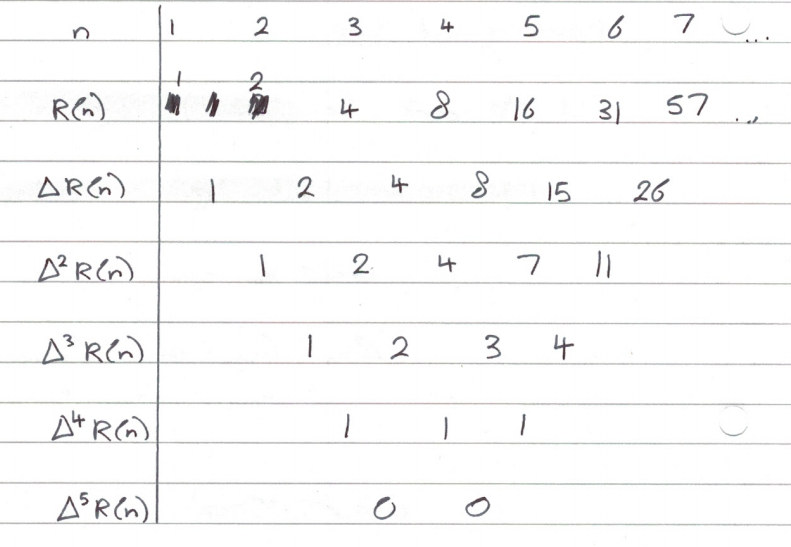
\includegraphics[scale=0.5]{differencetable}
\\\\
We say the above sequence $ R(n) $ is quartic, since the $ \Delta^{4}R(n) $ terms are constant.
\\
To calculate the next number in the sequence $ R(n) $, we can add another $ 0 $ to the $ \Delta^{5} $ row and follow the pattern upwards.

\section{Fixed point iteration}

Fixed-point iteration is a method of finding an approximate solution to $ f(x) = 0 $ for some function $ f $. We rewrite $ f(x) = 0 $ as an iterative formula:
\begin{equation}
x_{n+1} = F(x_{n})
\end{equation}
for some function $ F $. Let $ a $ denote the value that $ x_{n} $ tends towards. The associated \textbf{fixed point} of this formula is the point $ (a, 0) $. The fixed point is also the point of intersection between the lines $ y = x $ and $ y = F(x) $.
\\\\
We let the error term $ \epsilon_{n} $ be defined as:
\begin{equation}
\epsilon_{n} = a - x_{n}
\end{equation}

\subsubsection*{Case 1: $ F'(a) \neq 0 $}

In this case we say the formula has linear convergence. The error in each iterate changes by a factor of $ F'(a) $:
\begin{equation}
\epsilon_{n+1} \approx \epsilon_{n} F'(a)
\end{equation}
Upon further expansion we get:
\begin{align}
\epsilon_{n+1} & \approx \epsilon_{n} F'(a) \\
& \approx \epsilon_{n-1} F'(a)^{2} \\
& \vdots \\
& \approx \epsilon_{0} F'(a)^{n+1}
\end{align}
It is easy to see that if $ |F'(a)| < 1 $, the error terms will get tend to $ 0 $ and the iterative formula will indeed converge to $ a $. If $ |F'(a)| > 1 $, the error terms get bigger and the formula diverges from $ a $.

\subsubsection*{Case 2: $ F'(a) = 0, F''(a) \neq 0 $}

In this case the formula has quadratic convergence.
\begin{equation}
\epsilon_{n+1} \approx \frac{\epsilon_{n}^{2}}{2} F''(a)
\end{equation}
In this case we can see that for convergence, we must have $ |F''(a)| < 1 $.

\subsection{Newton-Raphson method}

The Newton-Raphson method is a special case of fixed-point iteration. The Newton-Raphson iterative formula to find a solution to $ f(x) = 0 $ is given by:
\begin{equation}
x_{n+1} =x_{n} - \frac{f(x_{n})}{f'(x_{n})}
\end{equation}
Newton-Raphson always converges quadratically, however it will only converge in specific situations (e.g. when there are no stationary points in between $ x_{0} $ and $ a $).

\section{Partial differentation and vector calculus}

\subsection{Exact equations}
Let us say we have an ODE of the form:
\begin{equation}
P(x, y) + Q(x, y)\frac{dy}{dx} = 0
\end{equation}
(note the coefficients are multi-variable functions). This can be rewritten as:
\begin{equation} \label{exactdifferential}
P(x, y) dx + Q(x, y) dy = 0
\end{equation}
We can try the exact equations method. We say an equation is exact iff:
\begin{equation}
\frac{\partial P}{\partial y} \equiv \frac{\partial Q}{\partial x} 
\end{equation}
This simple condition implies some important results. It can be shown that an exact equation implies the LHS of equation \ref{exactdifferential} is an exact (total) differential). This means it can be written as $ df $, where f is some function of $ x $ and $ y $. But the equation of this total differential is:
\begin{equation}
df = \frac{\partial f}{\partial x}dx + \frac{\partial f}{\partial y}dy
\end{equation}
Comparing to equation \ref{exactdifferential} we can note 3 things:
\begin{equation}
\begin{split}
P(x, y) & = \frac{\partial f}{\partial x} \\
Q(x, y) & = \frac{\partial f}{\partial y} \\
df & = 0
\end{split}
\end{equation}
We integrate $ P(x, y) $ w.r.t $ x $ and $ Q(x, y) $ w.r.t $ y $ and 'merge' the two expressions together (i.e. for any matching terms, write them down only once) to give us an expression for $ f(x, y) $. Ignore constants of integration. $ df = 0 $ tells us that $ f(x, y) = c $ by integration. Therefore the general solution is given by:
\begin{equation}
f(x, y) = c
\end{equation}
for some arbitrary constant c.

\newpage
\part{Linear Algebra}

\section{Definitions}

\paragraph{$ \R^{n} $}
The set of all column vectors with height $ n $.

\paragraph{Zero vector}
A column vector with all $ n $ entries $ 0 $. Denoted by $ \vec{0}_{n} $.

\paragraph{Standard basis vectors of $ \R^{n} $}
The set of column vectors with $ n $ entries, with a single entry as $ 1 $ and the rest $ 0 $.

\paragraph{Linear combination}
A linear combination of vectors $ \vec{v}_{1}...\vec{v}_{n} $ is an expression:
\begin{equation}
\lambda_{1} \vec{v}_{1} + \lambda_{2} \vec{v}_{2} + ... + \lambda_{n} \vec{v}_{n}
\end{equation}
where $ \lambda_{1}...\lambda_{n} \in \R $.

\paragraph{Span}
The span of of a set of vectors is the set of all linear combinations of those vectors.

\paragraph{Dot product}
The dot product of $ \vec{v} = \begin{pmatrix}
v_{1} \\ \vdots \\ v_{n}
\end{pmatrix} $ and $ \vec{u} = \begin{pmatrix}
u_{1} \\ \vdots \\ u_{n}
\end{pmatrix} $ is defined as:
\begin{equation}
\vec{v} \cdot \vec{u} = v_{1} u_{1} + v_{2} u_{2} + ... + v_{n} u_{n}
\end{equation}

\paragraph{Norm}
The norm (aka length) of a vector $ \vec{v} = \begin{pmatrix}
v_{1} \\ \vdots \\ v_{n}
\end{pmatrix} $ in $ \R^{n} $ is defined by:
\begin{equation}
||\vec{v}|| = \sqrt{\sum_{i=1}^{n} v_{i}^{2}}
\end{equation}

\paragraph{Unit vector}
Any $ \vec{v} $ such that $ ||\vec{v}|| = 1 $.

\paragraph{Zero matrix}
An $ m \times n $ matrix with all entries 0. Denoted by $ \vec{0}_{m \times n} $.

\paragraph{Transpose}
The transpose of a matrix $ \vec{A} $ is the result of flipping all rows with columns and vice versa. Denoted by $ \vec{A}^{T} $.

\paragraph{$ (a_{ij}) $ notation}
For an $ m \times n $ matrix $ \vec{A} $, we can say $ \vec{A} = (a_{ij}) $ if we represent the matrix as:
\begin{equation}
\begin{pmatrix}
a_{11} & a_{12} & \cdots & a_{1j} & \cdots & a_{1n} \\
a_{21} & a_{22} & \cdots & a_{2j} & \cdots & a_{2n} \\
\vdots & \vdots & \ddots & \vdots &        & \vdots \\
a_{i1} & a_{i2} & \cdots & a_{ij} & \cdots & a_{in} \\
\vdots & \vdots &        & \vdots & \ddots & \vdots \\
a_{m1} & a_{m2} & \cdots & a_{mj} & \cdots & a_{mn}
\end{pmatrix}
\end{equation}
\\
$ i $ denotes the row number and $ j $ denotes the column number. Hence we have $ 1 \leq i \leq m $ and $ 1 \leq j \leq n $.

\paragraph{Leading diagonal}
Let $ \vec{A} = (a_{ij}) $. The leading diagonal is made up of all entries of the form $ a_{ii} $, e.g. $ a_{11}, a_{22}, $ etc.

\paragraph{Identity matrix}
A square $ n \times n $ matrix where the leading diagonal is all $ 1 $s and the rest of the entries are $ 0 $. Denoted by $ I_{n} $.

\paragraph{Linear equation}
A linear equation of variables $ x_{1}...x_{n} \in \R $ is given by:
\begin{equation}
\lambda_{1} x_{1} + \lambda_{2} x_{2} + ... + \lambda_{n} x_{n} = b
\end{equation}
where $ \lambda_{1} ... \lambda_{n}, b \in R $.

\paragraph{System of linear equations}
A system of linear equations is a set of simultaneous linear equations.

\paragraph{Free variable}
A variable in a system of linear equations that can be set to any value, without affecting the validity of the solution.

\paragraph{Basic variable}
Any variable that is not a free variable (i.e. a solution only exists for particular values of this variable).

\paragraph{Augmented matrix}
For a system of linear equations represented as $ \vec{A} \vec{x} = \vec{b} $, the augmented matrix is $ (\vec{A} \ | \ \vec{b}) $. This is the matrix $ \vec{A} $ but with $ \vec{b} $ added in as an extra column on the right.

\paragraph{Row operation}
There are 3 types of row operation:
\begin{itemize}
\item Swapping rows
\item Multiplying a row by a scalar value
\item Adding a multiple of one row to another
\end{itemize}

\paragraph{Leading entry}
The leading entry of a row is the first non-zero entry in that row.

\paragraph{Row echelon form}
A matrix is in row echelon form if:
\begin{itemize}
\item All non-zero rows are above rows of all zeroes
\item Each leading entry is $ 1 $, and is in a column to the right of the leading entry in the row above
\item All entries in the column below a leading entry are $ 0 $
\end{itemize}
Note that any matrix in row echelon form is upper triangular.

\paragraph{Reduced row echelon form (RREF)}
A matrix is in reduced row echelon form if:
\begin{itemize}
\item The matrix is in reduced echelon form
\item Each leading entry is the only non-zero entry in its column
\end{itemize}
Any matrix in RREF is upper AND lower triangular.

\paragraph{Upper triangular}
A matrix is upper triangular if $ a_{ij} = 0 $ for $ i > j $.
\\
i.e. only the top-right half contains non-zero entries.

\paragraph{Strictly upper triangular}
A matrix is strictly upper triangular if $ a_{ij} = 0 $ for $ i \geq j $.

\paragraph{Lower triangular}
A matrix is lower triangular if $ a_{ij} = 0 $ for $ i < j $.
\\
i.e. only the bottom-left half contains non-zero entries.

\paragraph{Strictly lower triangular}
A matrix is strictly lower triangular if $ a_{ij} = 0 $ for $ i \leq j $.

\paragraph{Diagonal matrix}
A diagonal matrix is such that $ a_{ij} = 0 $ if $ i \neq j $.
\\
i.e. Only the leading diagonal contains non-zero entries.

\paragraph{Inverse}
The inverse of an $ n \times n $ matrix $ \vec{A} $ is such that:
\begin{equation}
\vec{A}^{-1} \vec{A} = \vec{A} \vec{A}^{-1} = I_{n}
\end{equation}
Note that this is one of the only occasions where matrix multiplication is commutative. Not all matrices have inverses.

\paragraph{Singular}
A matrix is called singular if it is non-invertible.

\paragraph{Determinant}
A specific number calculated from the entries in a matrix. Used in computing inverses. Denoted by $ \det(A) $.

\paragraph{Elementary matrix}
A matrix that differs from the identity matrix by one row operation.

\paragraph{Eigenvalue}
An eigenvalue of a matrix $ \vec{A} $ is some $ \lambda \in R $ that satisfies:
\begin{equation}
\vec{A} \vec{v} = \lambda \vec{v}
\end{equation}
for some $ \vec{v} \in \R^{n} $, called the eigenvector.

\paragraph{Eigenvalue}
An eigenvector of a matrix $ \vec{A} $ is some $ \vec{v} \in R^{n} $ that satisfies:
\begin{equation}
\vec{A} \vec{v} = \lambda \vec{v}
\end{equation}
for some $ \lambda \in \R $, called the eigenvalue.

\section{Theorems}



\end{document}